\chapter{Introduction}

Le projet a pour but de reproduire le jeu des amazones, célèbre pour sa richesse stratégique. C’est un jeu de plateau où le but de chaque joueur est de réduire les déplacements de l'adversaire tout en optimisant les siens et en apportant des modifications au terrain à chaque tour. 

\section{Règles}

\begin{itemize}
    \item[\textdagger] Déplacements : chaque pion, appelé reine, possède la même couverture de mouvement que la reine aux échecs.
    \medbreak
    \item [\textdagger] Tir : à la fin de chaque déplacement, la reine en question doit tirer une flèche dans une de la direction accessible par cette dernière.
    \medbreak
    \item [\textdagger] Condition de victoire : Le jeu termine lorsque toutes les reines d’un des deux joueurs ne sont plus en capacités de bouger.
    \medbreak
    \item [\textdagger] Client : Le jeu doit être réalisé de telle sorte que notre stratégie puisse être extraite afin de jouer une partie contre un autre adversaire sur son propre serveur.
    \medbreak
    \item [\textdagger] Serveur : le jeu doit également pouvoir faire jouer d'autres stratégies de provenance d'autres groupes de projet. Pour cela, certaines conventions ainsi que des vérifications anti-triche doivent être mises en place.
\end{itemize}

\section{Stratégie de résolution du sujet}

Ce projet est divisé en deux facettes, le développement des \textit{clients} et du \textit{serveur}. Il est indispensable que les clients soient automatiques et implémentent l'interface définie dans le sujet afin d'être compatible avec l'ensemble des serveurs utilisant celle-ci. Le travail a donc été réparti en conséquence entre client et serveur afin d'avoir un jeu qui fonctionne aussi bien en serveur local que sur un serveur externe.\\
Afin d'avoir un client constamment opérationnel, l'utilisation de la méthode de programmation par les tests a été mis en place pour le développement de ce dernier. Les tests ont donc été développés en amont afin de faire progresser le client petit à petit en résolvant les tests imposés.

\section{Architecture du projet}

Le projet se base sur la méthode d'implémentation et de représentation de graphe ainsi que de l'interaction client serveur. On remarque donc sur graphe de dépendance figure \ref{fig:my_label} que les fichiers posant les bases de l'environnement sont à la base du projet. Ensuite vient le client, qui ne dépend que peu de fichiers, car il se doit d'être malléable afin de s'adapter lors de son exportation sur des mondes différents, lors de l'exportation vers un autre serveur. \\
En haut de ce graphe, on retrouve le serveur qui est en quelque sorte celui qui lie réellement tous les fichiers ensemble et permet le fonctionnement du jeu. On retrouve en lui notamment la boucle de jeu ainsi que la création du monde et bien entendu les différents joueurs. C'est lui qui utilise toutes les fonctions de mouvements et de validations des coups. \\
Quant au fichier \texttt{tools}, lui, il sert davantage dans la partie test afin d'afficher les matrices GSL facilement.

\medbreak

\begin{figure}[H]
    \centering
    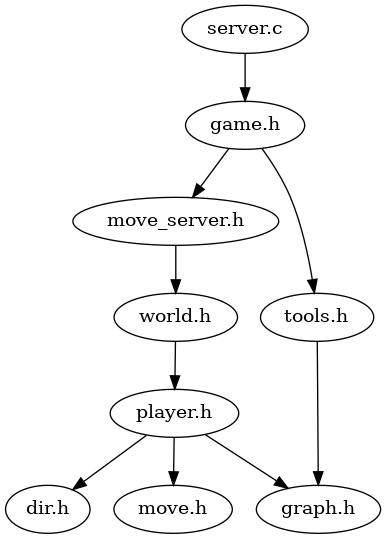
\includegraphics[scale=0.5]{dependency.png}
    \caption{Graph de dépendance du projet}
    \label{fig:my_label}
\end{figure}

\medbreak

Pour garantir le bon fonctionnement des implémentations tout au long du projet, des tests ont étés mis en place. Ces tests sont divisés en plusieurs fichiers, chacun étant destiné à tester un fichier précis du projet.